\chapter{Estado da Arte}
Esta parte se focará nas mais modernas tecnologias e técnicas para a realização da localização de ativos em um ambiente. Em primeiro lugar é importante fazer uma diferenciação entre a localização de ativos em ambientes outdoor e indoor.

A localização indoor é o termo dado para a localização em ambientes com muitos obstáculos, paredes e teto. Em contraste, o localização outdoor, acontece em ambientes abertos com poucos obstáculo e paredes. Justamente, por introduzir obstáculos, a localização indoor apresenta mais desafios em relação à outdoor. O ambiente em que o trabalho será feito, é um porto a céu aberto, entretando diversos obstáculos e paredes fazem parte desse ambiente, fazendo do problema mais similar com problemas de localização indoor. geralmente, soluções de localização indoor precisam tomar mais cuidado com precisão, economia de energia, alcançe limitado e interferências. Aspectos os quais serão necessários no problema em questão. Tais técnicas, em ambientes sem o obstáculo a mais imposto por um teto, podem alcançar resultados ainda melhores. Desse forma, a partir de agora, o texto se focará mais no estado-da-arte de tecnologias e técnicas desenvolvidas para ambientes indoor que serão as necessárias para esse trabalho.

\section{Tecnicas de localização}
Existe uma variedade de tecnicas e algoritmos para obter informações a partir das propriedades de um sinal recebido por um receptor. Os algoritmos usados em sistemas de localização, traduzem as propriedades de um sinal recebido em distâncias e ângulos, os quais são posteriormente usados para o cálculo da localização real de um determinado objeto [8]. Abaixo uma imagem que resume as principais propriedades de sinal analisadas e os principais algoritmos utilizados para a localização:

\begin{figure}[H]
	\centering 
	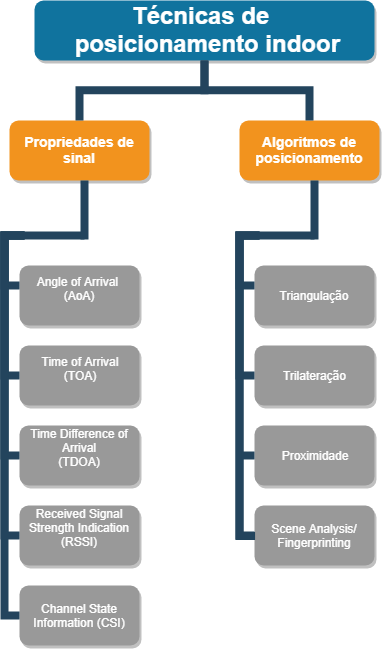
\includegraphics[scale = 0.4]{images/tecnicas_posicionamento_indoor.png}
	\caption{Técnicas localização indoor}
	\label{fig:tecnicas_posicionamento_indoor}
  \end{figure}


\subsection{Angle of Arrival}

Angle of Arrival (AoA), ou em português, angulo de chegada é o angulo em que o sinal transmitido chega ao receptor. Abordagens baseadas no AoA, usam matrizes de antenas e exploram a diferença de fase das ondas recebidas em cada elemento dessa matriz. E com tal informação é possivel estimar o AoA. Na figura \ref{fig:angle_of_arrival} mostra-se uma representação gráfica do processo.

Essa abordagem para estimativa do ângulo de chegada do sinal, geralmente envolve um hardware mais sofisticado quando em comparação com outras propriedades do sinal. Entretanto, com a informação do ângulo de chegada, algoritmos conseguem estimar uma localização com muito mais precisão.\cite{art1}

\begin{figure}[H]
	\centering 
	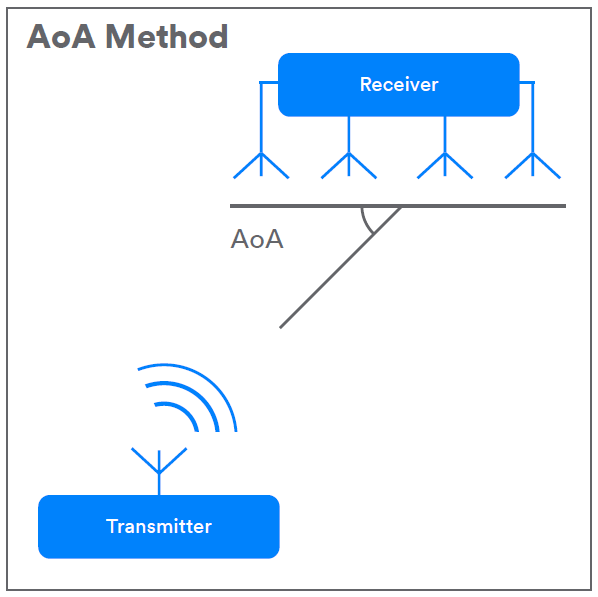
\includegraphics[scale = 0.6]{images/angle_of_arrival.png}
	\caption{Angle of Arrival (AoA)}
	\label{fig:angle_of_arrival}
\end{figure}

\subsection{Time of Arrival}

Time of Flight (ToF) também chamado de Time of Arrival (ToA) é uma técnica que explora o tempo trascorrido para o sinal emitido pelo transmissor chegar ao receptor. Multiplicando-se esse tempo pela velocidade de propagação da luz \(c = 3 \cdot 10^8\) é possivel achar a distância entre o sinal recebido e o sinal trasnmitido. Entretando essa técnica ainda não é muito precisa, devido as dimesões muito pequenas de tempo envolvidas em aplicaçãoes de curta distância. [9]

\subsection{Time Difference of Arrival (TDOA)}


